As our implementation description should make clear, we felt that we were able to express the rock slicing computations cleanly and elegantly using Spark's functional approach of constructing and subsequently transforming reliable distributed datasets. However, while Spark features clean abstractions, we have found that there is a bit of a discrepancy between the model conveyed by these abstractions and the behavior of our algorithm in a parallel setting. A number of subtleties emerged when we began studying how our code would behave ``in the wild.''

\subsection{Seeding the Initial RDD}
Before we can begin processing discontinuities in parallel, we need to construct an initial RDD of rock blocks to get started. This will serve as the parent of all subsequent block RDDs in the algorithm. Thus, we process the first few joints from the input data locally at the driver node to seed an initial collection of blocks that are then converted to an RDD and distributed amongst workers nodes. This proceeds just like the parallel rock cutting described above: iterate through joints and apply a \texttt{flatMap} transformation in order to check for intersections and produce child blocks when necessary. The number of rock blocks that are produced locally before conversion to an RDD is a tunable parameter. We have typically tried to make the initial number of blocks equal to the number of desired partitions in the child RDDs produced by the slicing algorithm.

\subsection{Number of Partitions in RDD}
Another important factor in the performance of the rock slicing algorithm is the number of partitions in the rock block RDDs. This in turn determines the number of compute tasks shared amongst Spark workers and therefore influences the degree of parallelism we can achieve. There is a general tradeoff involving the number of partitions: too few partitions leads to a small number of tasks that can be scheduled, forcing workers to sit idle and causing underutilization, while too many partitions and thus a high number tasks can lead to excessive communication amongst nodes. One would then expect that the optimal number of RDD partitions is closely related to the number of available CPU cores. Indeed, the Spark developers recommend as a general rule that RDD partitions should be constructed such that there are 2 to 3 tasks per core \cite{sparkTuning}. Section 5 presents results from experiments testing the relationship between partition count and overall performance as well as the value of this recommendation.

\begin{figure}[h]
\centering
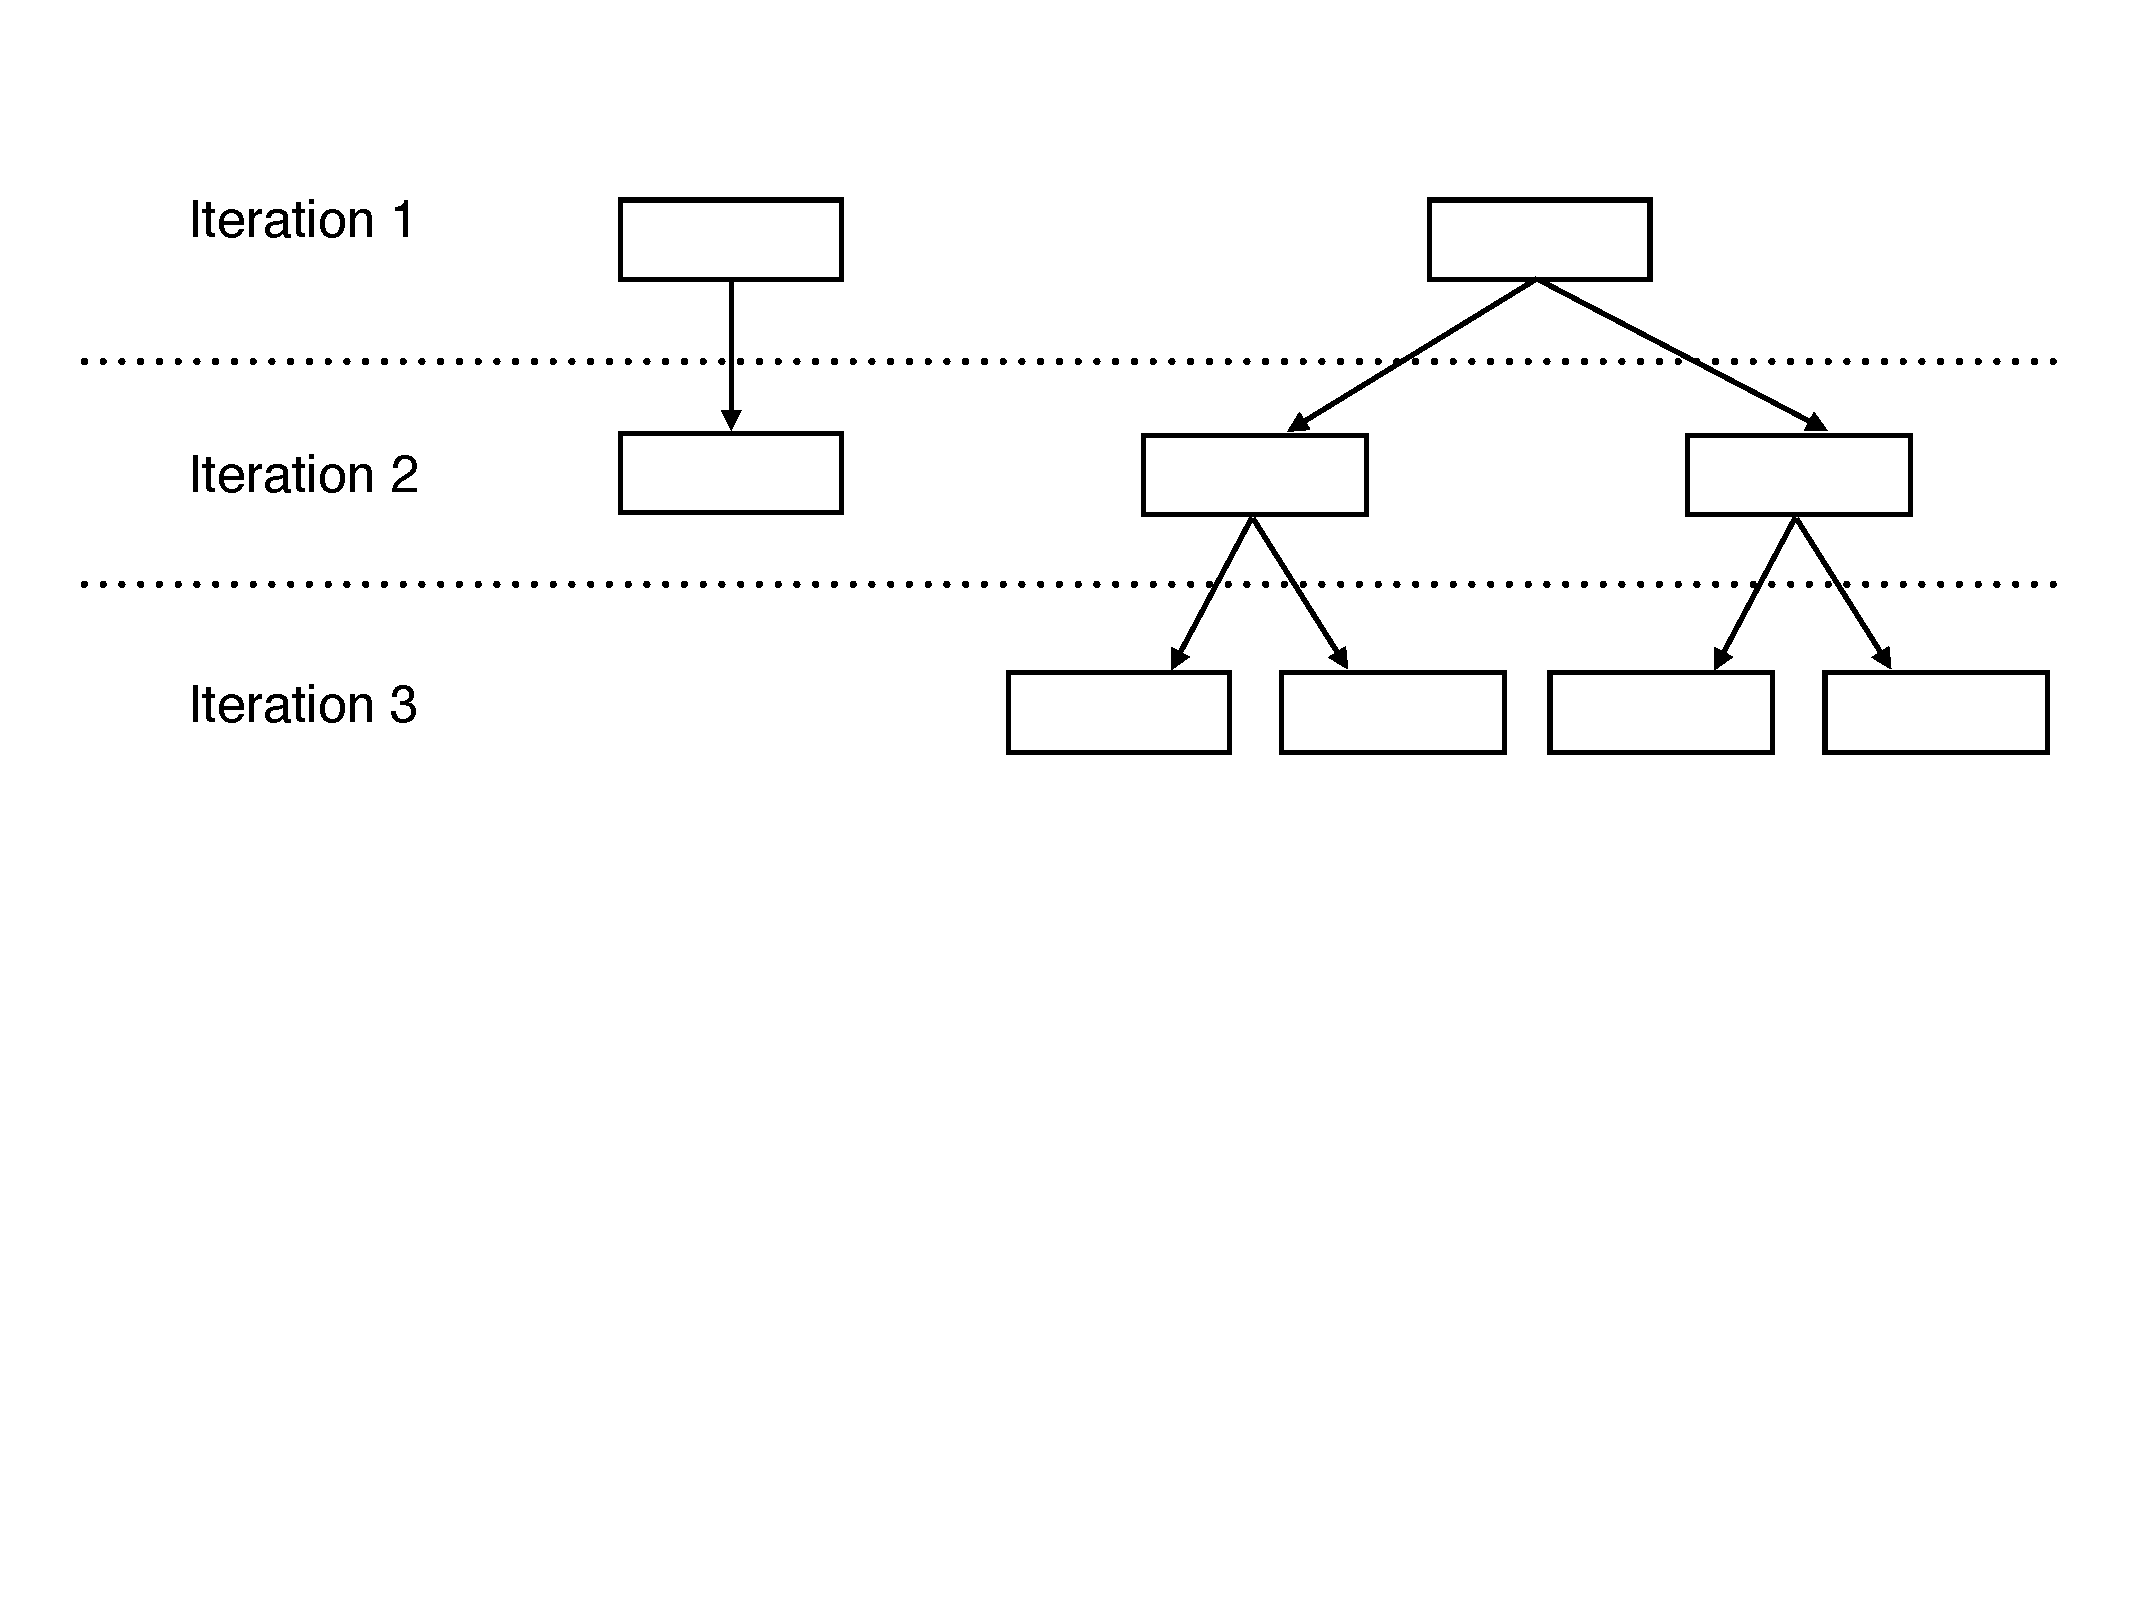
\includegraphics[width=0.4\textwidth]{flatMap.pdf}
\caption{An Example of Partition Imbalance Induced by Cutting Blocks}
\label{fig:flatMap}
\end{figure}

\subsection{Repartitioning to Avoid Data Skew}
We found data skew to be a major problem in the execution of our algorithm on Spark. Specifically, the sequence of \texttt{flatMap} transformations that perform the actual rock slicing can lead to large discrepancies in sizes of RDD partitions because the child blocks produced by cutting a parent block stay in the same RDD partition as the parent block by default, and cuts do not occur with equal frequency across partitions. In the example of Figure \ref{fig:flatMap}, we see how one RDD partition quadruples in size over two iterations, while the other partition remains the same. This imbalance means that some partition transformations require significantly more computing time than others, causing nodes that have completed compute tasks associated with the smaller partitions to sit idle while waiting for others to catch up. The resulting underutilization can significantly impact the running time of our algorithm.

There are two potential approaches that could mitigate this problem. Assuming that discontinuities are distributed uniformly throughout the rock volume, we could attempt to generate an initial RDD of blocks that each cover a roughly equal volume. The partitions that arise as the blocks and their children are cut would then remain roughly equal in size. Unfortunately, this is not a feasible approach in our domain because the distribution of discontinuities is rarely uniform throughout the entire rock volume. More importantly, the order in which joints are processed has important geological implications. It is generally best to process joints in descending order by age. That is, the older joints are processed before younger joints. This is especially important when joints could be non-persistent because older joints tend to cover a larger area, while younger joints might not even be meaningful until the adjacent rock blocks have been defined by cuts induced when processing older joints.

This forces us to apply a different approach: periodically repartitioning the rock block RDD as joints are processed in order to balance partition sizes. This can be a costly operation because it involves an all-to-all communication and data shuffle amongst Spark workers. This leads to yet another tradeoff: repartition too frequently and too much time will be used for communication and shuffling data instead of more meaningful computations. However, if repartitioning isn't performed frequently enough, our algorithm suffers from the data skew described above. We include yet another parameter in our algorithm that specifies a repartitioning period: the number of joints that are processed (and hence the number of \texttt{flatMap} transformations performed) between repartitioning operations. We analyze the impact of repartitioning frequency on performance in the following section.
